% A4縦・1段組の学習用（教科書風）テンプレート
\documentclass[paper=a4,fleqn]{jlreq}
\special{papersize=\the\paperwidth,\the\paperheight}

\usepackage[margin=20truemm]{geometry}
\usepackage[dvipdfmx]{graphicx}
\usepackage{amsmath,amssymb}
\usepackage{tikz}
\usepackage{pgfplots}
\pgfplotsset{compat=1.18}
\usetikzlibrary{arrows.meta,calc,angles,quotes}

\ModifyHeading{section}{
  lines=1,
  before_space=14pt,
  after_space=6pt
}

\ModifyHeading{subsection}{
  lines=1,
  before_space=10pt,
  after_space=4pt
}

\title{学習プリントテンプレート（教科書風）}
\author{数学科}
\date{\today}

\begin{document}
\maketitle
\tableofcontents

\section{単元名：三角比の基本}
\subsection{このページの目標}
\begin{itemize}
  \item 直角三角形で $\sin,\cos,\tan$ の意味を説明できる。
  \item 辺の長さから三角比を求められる。
\end{itemize}

\subsection{導入}
直角三角形 $\triangle ABC$ （$\angle B = 90^\circ$）を考える。角 $\angle A = \theta$ とすると，
\[
\sin\theta = \frac{\text{対辺}}{\text{斜辺}},\quad
\cos\theta = \frac{\text{隣辺}}{\text{斜辺}},\quad
\tan\theta = \frac{\text{対辺}}{\text{隣辺}}
\]
で定義される。

\subsection{図で確認}
\begin{center}
\begin{tikzpicture}[scale=1.2]
  \coordinate (A) at (0,0);
  \coordinate (B) at (4,0);
  \coordinate (C) at (4,2.5);
  \draw (A)--(B)--(C)--cycle;
  \draw (4,0) rectangle (3.8,0.2);
  \draw (0.7,0) arc[start angle=0,end angle=32,radius=0.7];
  \node[right] at (0.95,0.4) {$\theta$};
  \node[below] at (2,0) {隣辺};
  \node[right] at (4,1.25) {対辺};
  \node[left] at (2.1,1.35) {斜辺};
\end{tikzpicture}
\end{center}

\subsection{例題}
辺の長さが $3,4,5$ の直角三角形で，角 $\theta$ を長さ4の辺に隣接する角とする。
\[
\sin\theta = \frac{3}{5},\quad
\cos\theta = \frac{4}{5},\quad
\tan\theta = \frac{3}{4}
\]

\subsection{確認問題}
\begin{enumerate}
  \item 直角三角形で，対辺が $6$，斜辺が $10$ のとき，$\sin\theta$ を求めよ。
  \item 対辺が $5$，隣辺が $12$ のとき，$\tan\theta$ を求めよ。
\end{enumerate}

\section{単元名：一次関数の見方}
\subsection{ポイント}
一次関数 $y=ax+b$ では，$a$ が傾き，$b$ が切片を表す。

\subsection{グラフ例}
\begin{center}
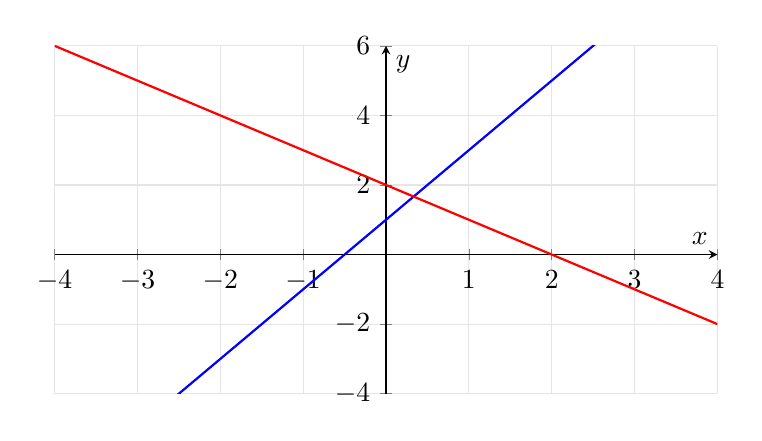
\begin{tikzpicture}
  \begin{axis}[
    width=10cm,
    height=6cm,
    axis lines=middle,
    xmin=-4,xmax=4,
    ymin=-4,ymax=6,
    xlabel={$x$},ylabel={$y$},
    grid=both,
    grid style={gray!20}
  ]
    \addplot[blue,thick,domain=-4:4]{2*x+1};
    \addplot[red,thick,domain=-4:4]{-x+2};
  \end{axis}
\end{tikzpicture}
\end{center}

\subsection{読み取り}
\begin{itemize}
  \item 青い直線の傾きは $2$，切片は $1$。
  \item 赤い直線の傾きは $-1$，切片は $2$。
\end{itemize}

\subsection{章末チェック}
\begin{enumerate}
  \item $y=-3x+4$ の傾きと切片を書け。
  \item 点 $(1,3)$ は $y=2x+1$ 上にあるか判定せよ。
\end{enumerate}

\end{document}
